\chapter{Einführung}
\label{sec:einfuehrung}

\section{Über den Autor}
\label{sec:einfuehrung:autor}
Mein Name ist Simon Lang. Als gelernter Informatiker arbeite ich seit 2006 in der Webentwicklungsbranche.
Seit 2012 studiere ich Informatik an der \Gls{zhawLabel}.
Durch mehrjährige Erfahrung in der Webentwicklung habe ich mich im Seminar zur Vorlesung \textit{Software Engineering} für die Vertiefung im Web entschieden.

\section{Aufbau}
Die Arbeit befasst sich mit den wesentlichen Schritten der Softwareentwicklung, welche im SWEBOK\footcite{IEEE_Computer_Society_2015-05-30} beschrieben sind.
\begin{itemize}
\item Requirements Engineering
\item Software Design
\item Software Construction
\item Software Testing
\item Software Maintenance / Software Configuration Management
\end{itemize}

Als Wissen wird vorausgesetzt, was die grundlegenden Arbeitsschritte in den einzelnen Kabiteln des SWEBOK sind. Die Arbeit geht nicht direkt über das SWEBOK, sondern befasst sich mit den speziellen Ausprägung für die Softwareentwicklung im Internet.

\section{Aufbau des Internets}
Das Internet ist eine Client/Server Architektur. Die Clients stellen Anfragen an einen Server, welcher eine Antwort zurückliefert. Der Client kann dabei ein Benutzer an seinem Computer sein, oder eine Maschine. In der Reisebranche ist dies zum Beispiel der Fall, wenn der Benutzer etwas bucht. Er bestätigt seinen Einkauf und der Server bucht darauf die Reise. Der Server verbindet sich dabei auf ein drittes System, zum Beispiel jenes des Reiseveranstalters. 

\begin{figure}[H]
  \centering
  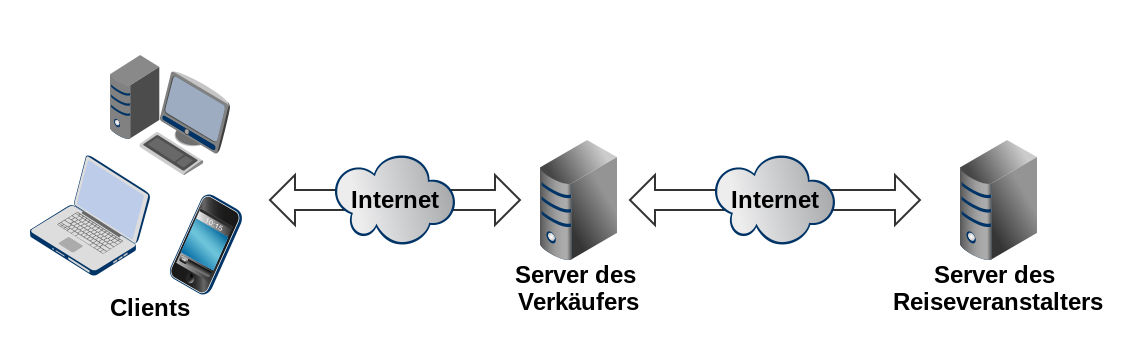
\includegraphics[width=0.9\textwidth]{images/aufbau-internet.png}
  \caption{Aufbau des Internet}
  \label{fig:einfuehrung:aufbau-des-internets}
\end{figure}

Wenn eine Webseite angezeigt werden soll, fragt der Client den Server an, und dieser liefert ein \Gls{glos:htmlLabel} Dokument aus. Dieses kann weitere Dokumente von weiteren Servern abfragen, wie zum Beispiel Bilder.
Das \Gls{glos:htmlLabel} Dokument wird von einer Programmiersprache auf dem Server generiert. Das ausgelieferte Dokument kann danach von einer Client-Seitigen Sprache weiter modifziert werden. Als Programmiersprache auf dem Client wird meistens \gls{jsLabel} eingesetzt. Die \Gls{glos:htmlLabel} Datei sollte nur den Inhalt und die Struktur der Webseite vorgeben. Das Aussehen wird über \gls{cssLabel} definiert.



\section{Standards}
Es gibt unzählige Standards für das \gls{wwwLabel}. Die wichtigsten werden vom \gls{w3cLabel}\footcite{World_Wide_Web_Consortium_2015-05-30} herausgegeben.
Die Standards sind folgendermassen strukturiert:
\begin{itemize}
\item Web Design and Applications
\item Web of Devices
\item Web Architecture
\item Semantic Web
\item XML Technology
\item Web of Services
\item Browsers and Authoring Tools
\end{itemize}
Vorgegeben wird die Sprache \Gls{glos:htmlLabel} und auch wie diese Dokumente aufgebaut werden sollen. Auch wie die Browser die Dateien darzustellen haben ist Teil eines Standards des \gls{w3cLabel}.

Seit einigen Jahren wurden die Standards für Mobiltelefone und Tablets erweitert. Programmierer für das Internet sollten die gängigsten Standards kennen und sich auch daran halten, so dass andere Entwickler sich einfacher in den bestehenden Code einarbeiten können.
